% 设定文章类型,正文字号为小四
\documentclass[zihao=-4,UTF8]{article}		

% 导入基本宏包
\usepackage[UTF8]{ctex}       % 设置文档为中文语言(中文paper留此行,删去上一行)
\usepackage{amsmath}    % 宏包:数学公式
\usepackage{amssymb}    % 宏包:提供更多数学符号

% 文章页面margin设置
\usepackage[a4paper]{geometry}
\geometry{top=1in}    % 1 inch= 2.46 cm, 0.75 inch = 1.85 cm
\geometry{bottom=1in}
\geometry{left=1.25in}  
\geometry{right=1.25in}   % 设置上下左右页边距
\geometry{marginparwidth=1.75cm}    % 设置边注距离(注释、标记等)

% 页眉页脚设置
\usepackage{fancyhdr}   %宏包:页眉页脚设置
\pagestyle{fancy}
\fancyhf{}
\cfoot{\thepage}
\renewcommand\headrulewidth{1pt}
\renewcommand\footrulewidth{0pt}
\chead{这里是页眉}    

% 外源代码插入设置
\usepackage{matlab-prettifier}
\lstset{
    style=Matlab-editor,  % 继承matlab代码颜色等
}
\usepackage[most]{tcolorbox} % 引入tcolorbox包 
\usepackage{listings} % 引入listings包
\tcbuselibrary{listings, skins, breakable}
\lstdefinestyle{matlabstyle}{
  language=Matlab,
  basicstyle=\small,
  breakatwhitespace=false,
  breaklines=true,
  captionpos=b,
  keepspaces=true,
  numbers=left,
  numbersep=15pt,
  showspaces=false,
  showstringspaces=false,
  showtabs=false,
  tabsize=2
}
\newtcblisting{matlablisting}{
  arc=0pt,
  top=0pt,
  bottom=0pt,
  left=1mm,
  listing only,
  listing style=matlabstyle,
  breakable,
  colback=white   % 选一个合适的颜色
}

% 图片插入自定义设置
\usepackage{graphicx}  % 宏包:图片插入
\usepackage{float}     
\usepackage{caption}
\captionsetup[figure]{name=图}  % 设置图标题为“图”以防出现“figure”
\captionsetup[table]{name=表}   % 设置表标题为“表”以防出现“table”
\captionsetup{labelfont=bf, font=small}   % 将表、图等标题设置为bf,字号为small(五号)
\usepackage[export]{adjustbox}           

% 文章默认字体设置
\usepackage{fontspec}   % 宏包:字体设置
\usepackage{xcolor}    % 宏包:更多颜色设置
\setmainfont{SimSun}    % 设置中文字体为宋体字体
\setmainfont{Times New Roman} % 设置英文字体为Times New Roman

% 参考文献引用设置
\bibliographystyle{unsrt}   % 设置参考文献引用格式为unsrt
\newcommand{\upcite}[1]{\textsuperscript{\cite{#1}}}     % 自定义上角标式引用
\renewcommand\refname{参考文献}  % 将参考文献标题改为中文(但似乎没有什么作用)

% 文章信息设置
\title{\textbf{这是文章的标题}}
\author{ }
\date{ }

% 表格美化设置
\usepackage{booktabs}

% title自定义设置
\usepackage{titling}  % 宏包:标题设置
\setlength{\droptitle}{-1.7cm}  % 调整标题位置
\pretitle{\begin{center}\LARGE}
\posttitle{\end{center}}

% 文档摘要设置
\newcommand{\cnabstractname}{\large 摘要}
\newenvironment{cnabstract}{%
  \par
  \noindent\mbox{}\hfill{\bfseries \cnabstractname}\hfill\mbox{}\par
  }{\par}
  
% 各级标题样式自定义
\usepackage{titlesec}
\titleformat{\section}{\large\centering\bfseries}{\thesection.}{1em}{}
\titleformat{\subsection}{\normalsize\bfseries}{\thesubsection}{1em}{}

 % 开始编辑文章
\begin{document}
\maketitle
\thispagestyle{fancy}
\vspace{-75pt}
\begin{cnabstract}
  {\normalsize 
  题目怎么这么样,本文怎么怎么样\par
  \textbf{对于问题一:}我们怎么怎么样\par
  \textbf{对于问题二:}我们怎么怎么样\par
  \textbf{对于问题三:}我们怎么怎么样\par
  \textbf{对于问题四:}我们怎么怎么样\par
  最后,我们综合什么什么,怎么怎么样
  }\par
  \vspace{12pt}
  {\normalsize \textbf{关键词:  关键字1,关键字2,关键字3}}
  \end{cnabstract}
\setlength{\parindent}{2em}

\newpage
\section{问题重述}
\subsection{问题背景:}
我查查查资料,然后说哇这个问题背景多好,多有研究意义,简直太棒了太棒了太棒了太棒了太棒了太棒了太棒了太棒了太棒了太棒了太棒了太棒了太棒了太棒了太棒了太棒了太棒了太棒了太棒了太棒了太棒了太棒了太棒了太棒了太棒了太棒了太棒了太棒了太棒了太棒了
\subsection{问题提出(题目重述):}
我重述重述再重述我重述重述再重述我重述重述再重述我重述重述再重述\par
根据上面的信息,我们提出以下几个问题:\par
\textbf{问题一:}这里是问题一\par
\textbf{问题二:}这里是问题二\par
\textbf{问题三:}这里是问题三\par
\textbf{问题四:}这里是问题四\par

\section{问题分析}
\subsection{问题一分析:}
这里我们分析问题一,提出我们将要的模型,给出解决问题的步骤,可以适当增加流程图、有利于问题分析的图像等(物理图解可以用PPT画,也可以用vscode插件draw.io画)。
\subsection{问题二分析:}
这里我们分析问题二,提出我们将要的模型,给出解决问题的步骤
\subsection{问题三分析:}
这里我们分析问题三,提出我们将要的模型,给出解决问题的步骤
\subsection{问题四分析:}
这里我们分析问题四,提出我们将要的模型,给出解决问题的步骤

\section{模型假设}
假设1:巴拉巴拉\par
假设2:巴拉巴拉\par
假设3:巴拉巴拉\par
假设4:芭芭拉巴拉\par
假设5:巴拉巴拉

\section{符号说明}
\begin{table}[ht]
  \centering
  \caption{\textbf{符号含义与约定}}
  \label{tab:waterpump}
  \begin{tabular}{ccccc}
  \toprule
  符号 & 符号含义& 单位\\
  \midrule
  符号1& 含义1& 单位1\\
  符号2& 含义2& 单位2\\
  符号3& 含义3& 单位3\\
  符号4& 含义4& 单位4\\
  \bottomrule
  \end{tabular}
\end{table}

\section{模型建立与求解}

\subsection{问题一:}
\subsubsection{模型建立:}
巴拉巴拉巴拉巴拉巴拉巴拉

\begin{figure}[H]
  \centering
  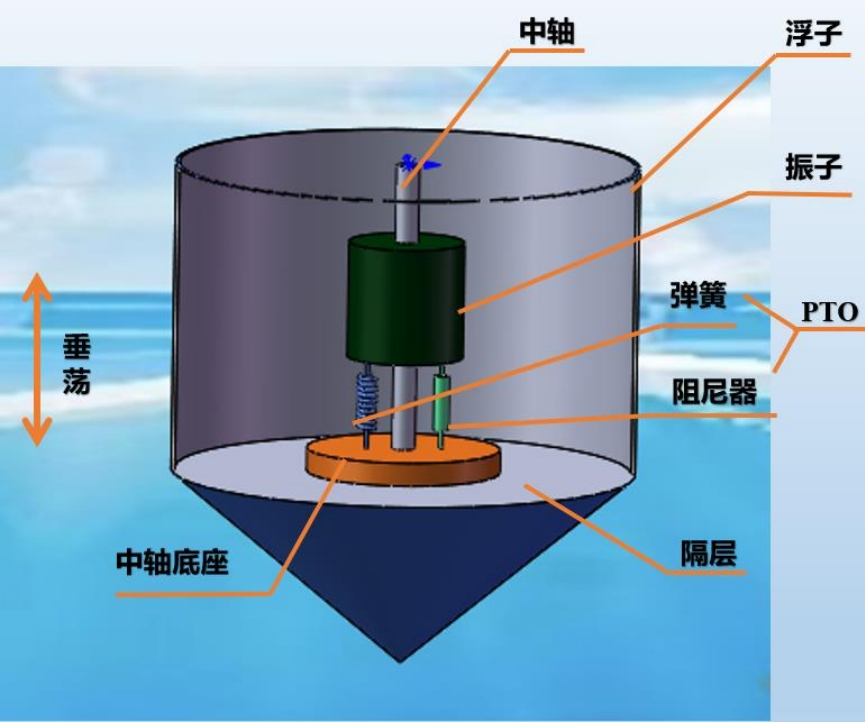
\includegraphics[width=0.6\textwidth]{assets/波浪能装置示意图.jpg}
  \caption{\textbf{插入 jpg}}\label{插入 jpg}
\end{figure}
啊?
\begin{figure}[H]
  \centering
  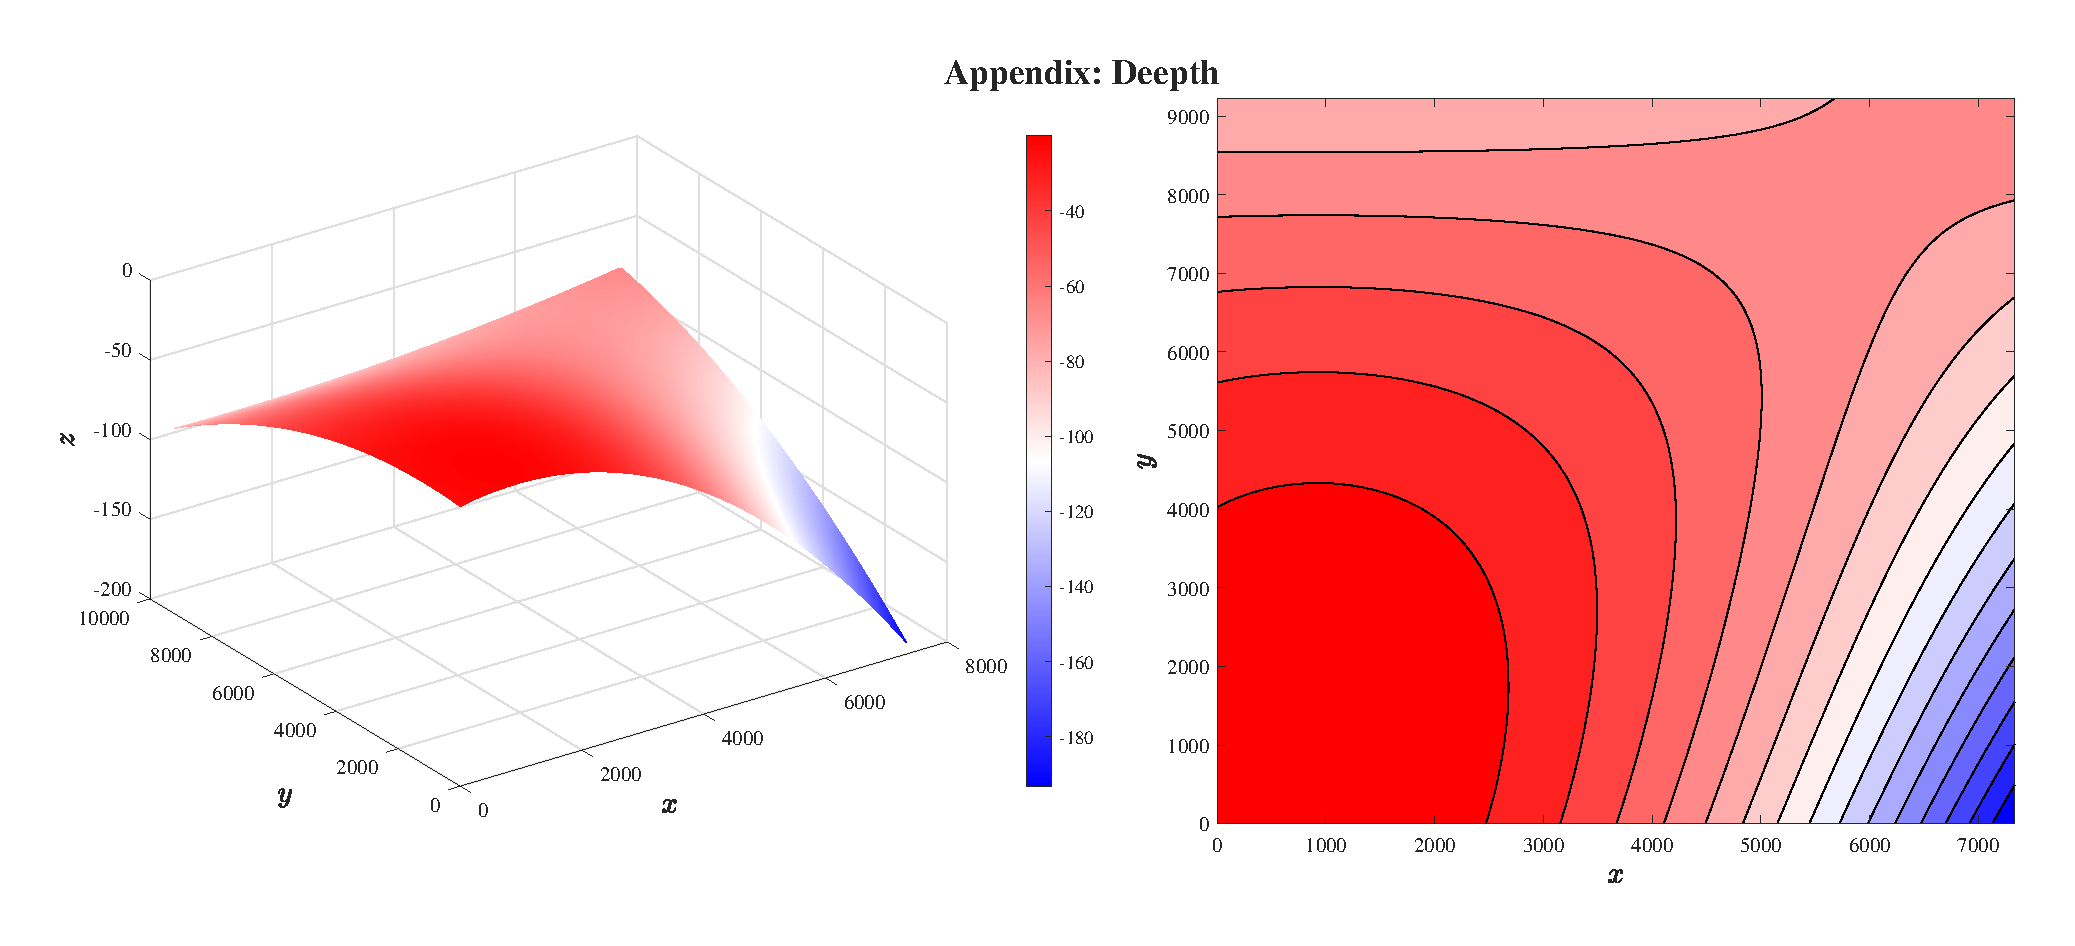
\includegraphics[width=\textwidth]{assets/2024-08-15_02-04-29.pdf}
  \caption{\textbf{插入 pdf}}\label{插入 pdf}
\end{figure}

\subsubsection{模型优化(如果可以优化的话):}
\subsubsection{模型求解:}
\subsubsection{求解结果:}
\subsubsection{可靠性检验:}

\subsection{问题二:}
\subsubsection{模型建立:}
使用巴拉巴拉
\subsubsection{模型求解:}

\begin{figure}[H]
  \centering
  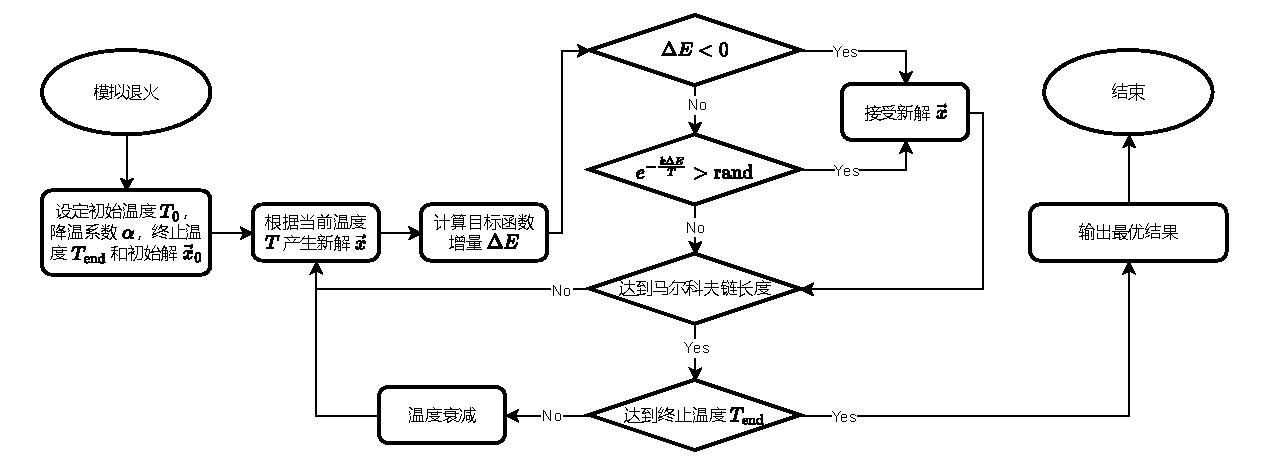
\includegraphics[width=\textwidth]{assets/模拟退火流程图.drawio.pdf}
  \caption{\textbf{模拟退火流程图}}\label{模拟退火流程图}
\end{figure}

\begin{figure}[H]
  \centering
  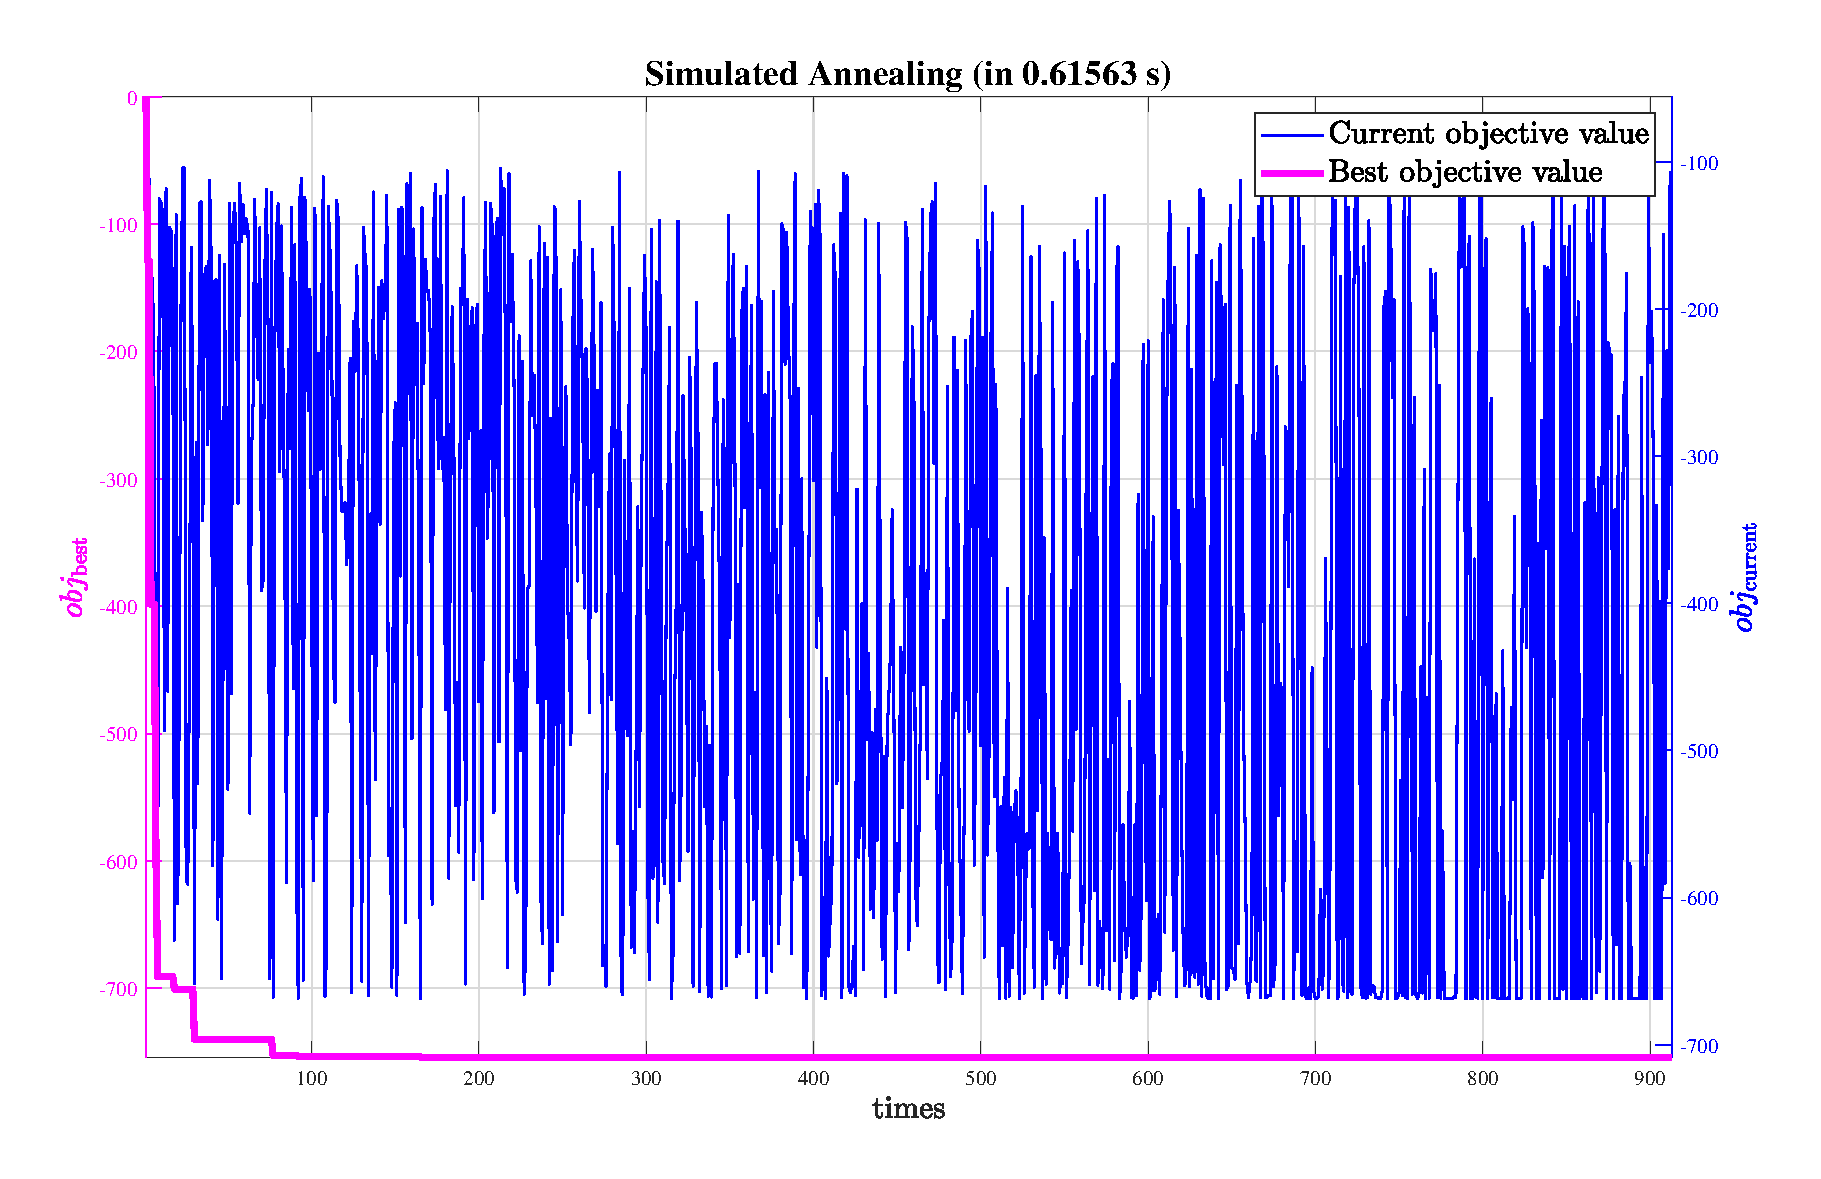
\includegraphics[width=\textwidth]{assets/2024-08-15_13-50-23.pdf}
  \caption{\textbf{模拟退火结果}}\label{模拟退火结果}
\end{figure}

\subsubsection{求解结果:}
\subsubsection{可靠性检验:}

\subsection{问题三:}
\subsubsection{模型建立:}
使用巴拉巴拉
\subsubsection{模型求解:}
\subsubsection{求解结果:}
\subsubsection{可靠性检验:}

\subsection{问题四:}
\subsubsection{模型建立:}
使用巴拉巴拉
\subsubsection{模型求解:}
我解解解解解解解解解解解解解解解解解解解解
\subsubsection{求解结果:}
这里是我们的求解结果
\subsubsection{可靠性检验:}

\section{模型评价与推广}
\subsection{模型优点:}
\subsubsection{优点一:}
\subsubsection{优点二:}
\subsection{模型缺点:}
\subsubsection{缺点一:}
\subsubsection{缺点二:}
\subsection{模型推广:}

\nocite{*}
\bibliography{re}
\thispagestyle{fancy} 
\addcontentsline{toc}{section}{参考文献}


\newpage
\appendix
\titleformat{\section}{\large\centering\bfseries}{附录\thesection.}{1em}{}
\titleformat{\subsection}{\normalsize\bfseries}{\thesubsection}{1em}{}

\section{支撑材料列表}
\begin{center}
  这里插入一张图片(类似思维导图那种)
\end{center}
\section{这里是我的第二节附录}
% 注意:listing环境中手动输入的代码需要顶格写

\begin{matlablisting}
% MATLAB code here
x = 0:0.1:2*pi;
y = sin(x);
plot(x, y);
xlabel('x');
ylabel('sin(x)');
title('Sine Function');
% ... (MATLAB code here,最好是插入文件)
% MATLAB code here
x = 0:0.1:2*pi;
y = sin(x);
plot(x, y);
xlabel('x');
ylabel('sin(x)');
title('Sine Function');
% ... (MATLAB code here,最好是插入文件)
% MATLAB code here
x = 0:0.1:2*pi;
y = sin(x);
plot(x, y);
xlabel('x');
ylabel('sin(x)');
title('Sine Function');
% ... (MATLAB code here,最好是插入文件)
% MATLAB code here
x = 0:0.1:2*pi;
y = sin(x);
plot(x, y);
xlabel('x');
ylabel('sin(x)');
title('Sine Function');
% ... (MATLAB code here,最好是插入文件)
% MATLAB code here
x = 0:0.1:2*pi;
y = sin(x);
plot(x, y);
xlabel('x');
ylabel('sin(x)');
title('Sine Function');
% ... (MATLAB code here,最好是插入文件)
% MATLAB code here
x = 0:0.1:2*pi;
y = sin(x);
plot(x, y);
xlabel('x');
ylabel('sin(x)');
title('Sine Function');
% ... (MATLAB code here,最好是插入文件)% ... (MATLAB code here,最好是插入文件)% ... (MATLAB code here,最好是插入文件)% ... (MATLAB code here,最好是插入文件)% ... (MATLAB code here,最好是插入文件)A
% MATLAB code here
x = 0:0.1:2*pi;
y = sin(x);
plot(x, y);
xlabel('x');
ylabel('sin(x)');
title('Sine Function');
% ... (MATLAB code here,最好是插入文件)
\end{matlablisting}

\section{这里是我的第三节附录}
\end{document}

